\documentclass{article}
\usepackage[utf8]{inputenc}
\usepackage[T1]{fontenc}
\usepackage[finnish]{babel}
\usepackage{graphicx}
\usepackage{amssymb}

\title{Van Aubelin lause}
\author{Kandidaatintutkielma\\Maria Larionova}
\date{\today}

\begin{document}
\maketitle
\pagebreak
\tableofcontents
\pagebreak

\section{Johdanto}
Van Aubelin lause osoittaa nelikulmioiden sivuun piirrettävien neliöiden ominaisuuden. Minkä tahansa nelikulmion jokaista sivua kohti piirretään neliö, jonka sivujen pituudet ovat saman pituisia kuin sen nelikulmion sivun pituus, johon neliö yhtyy. Tällaisten neliöiden keskipisteistä piirretään vastakkaiseen neliön keskipisteeseen jana. Van Aubelin lauseen mukaan, nämä janat ovat yhtä pitkiä ja leikkaavat toisensa kohtisuorassa. 

Lause on nimetty H. H. van Aubelin mukaan, joka julkaisi todistuksen vuonna 1878.

\pagebreak
\section{Esitiedot}
Todistuksessa tulemme käyttämään yhteneviä kolmiota, niiden määritelmää ja ominaisuuksia, nämä tiedot oletan esitiedoiksi. Tämän lisäksi käytämme kolmion sivuille piirrettyjen neliöiden ominaisuutta. Koska tämä ei ole niin itsestään selvää niin avaan lausetta ja todistan sen lyhyesti.

\pagebreak
\section{Todistus}
Lause voidaan todistaa joko vektorien tai geometrian avulla. Tässä esittelen todistuksen, joka on tehty geometrian avulla käyttäen yhteneviä kolmioita.

\textbf{Lause:} Suorakulman sivuille piirretyistä neliöiden keskipisteistä yhdistetyt janat vastakkaiseen nelikulmioon ovat yhtä pitkät ja toisiaan kohtaan kohtisuorassa. 
\begin{center}
    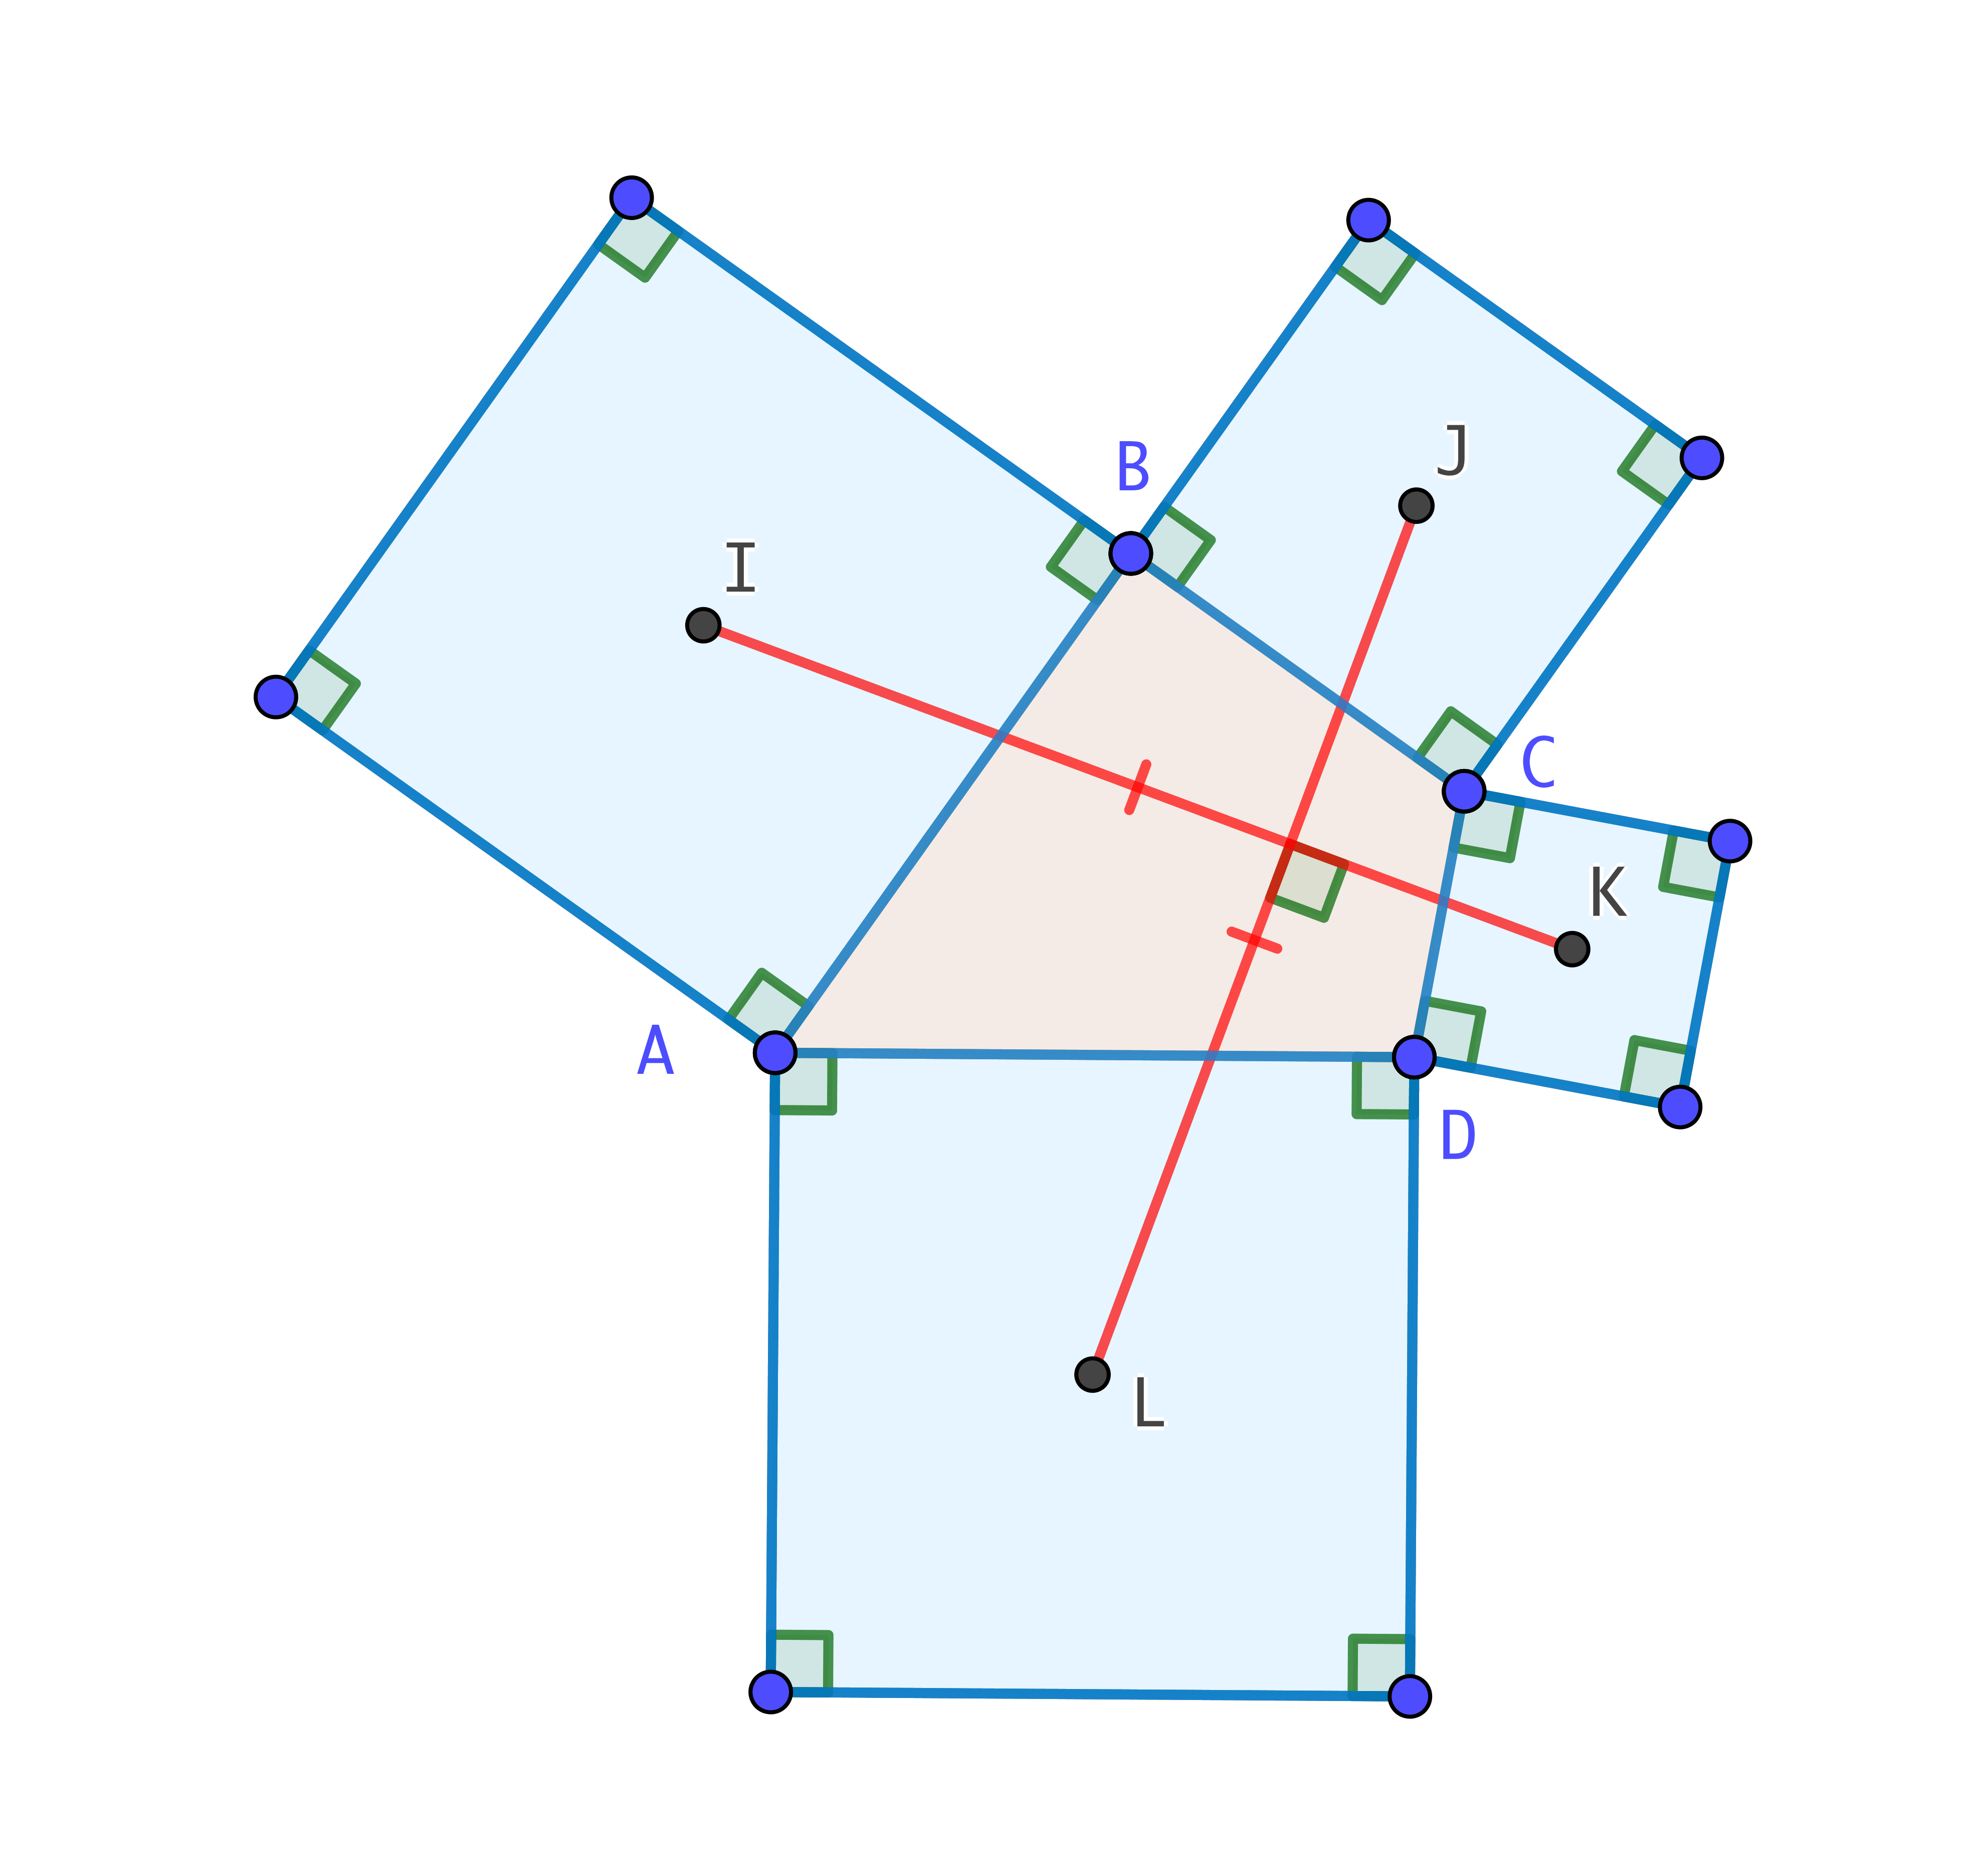
\includegraphics[scale=0.3]{todistuskuva}
\end{center}

\textbf{Todistus:} Valitaan suorakulmion lävistäjältä AC keskipiste M. Piirretään janat IM ja JM. Nämä janat muodostavat suoran kulman aikaisemmin todistetun lauseen mukaan. Samoin muodostetaan janat LM ja KM, niillä on sama ominaisuus.
\begin{center}
    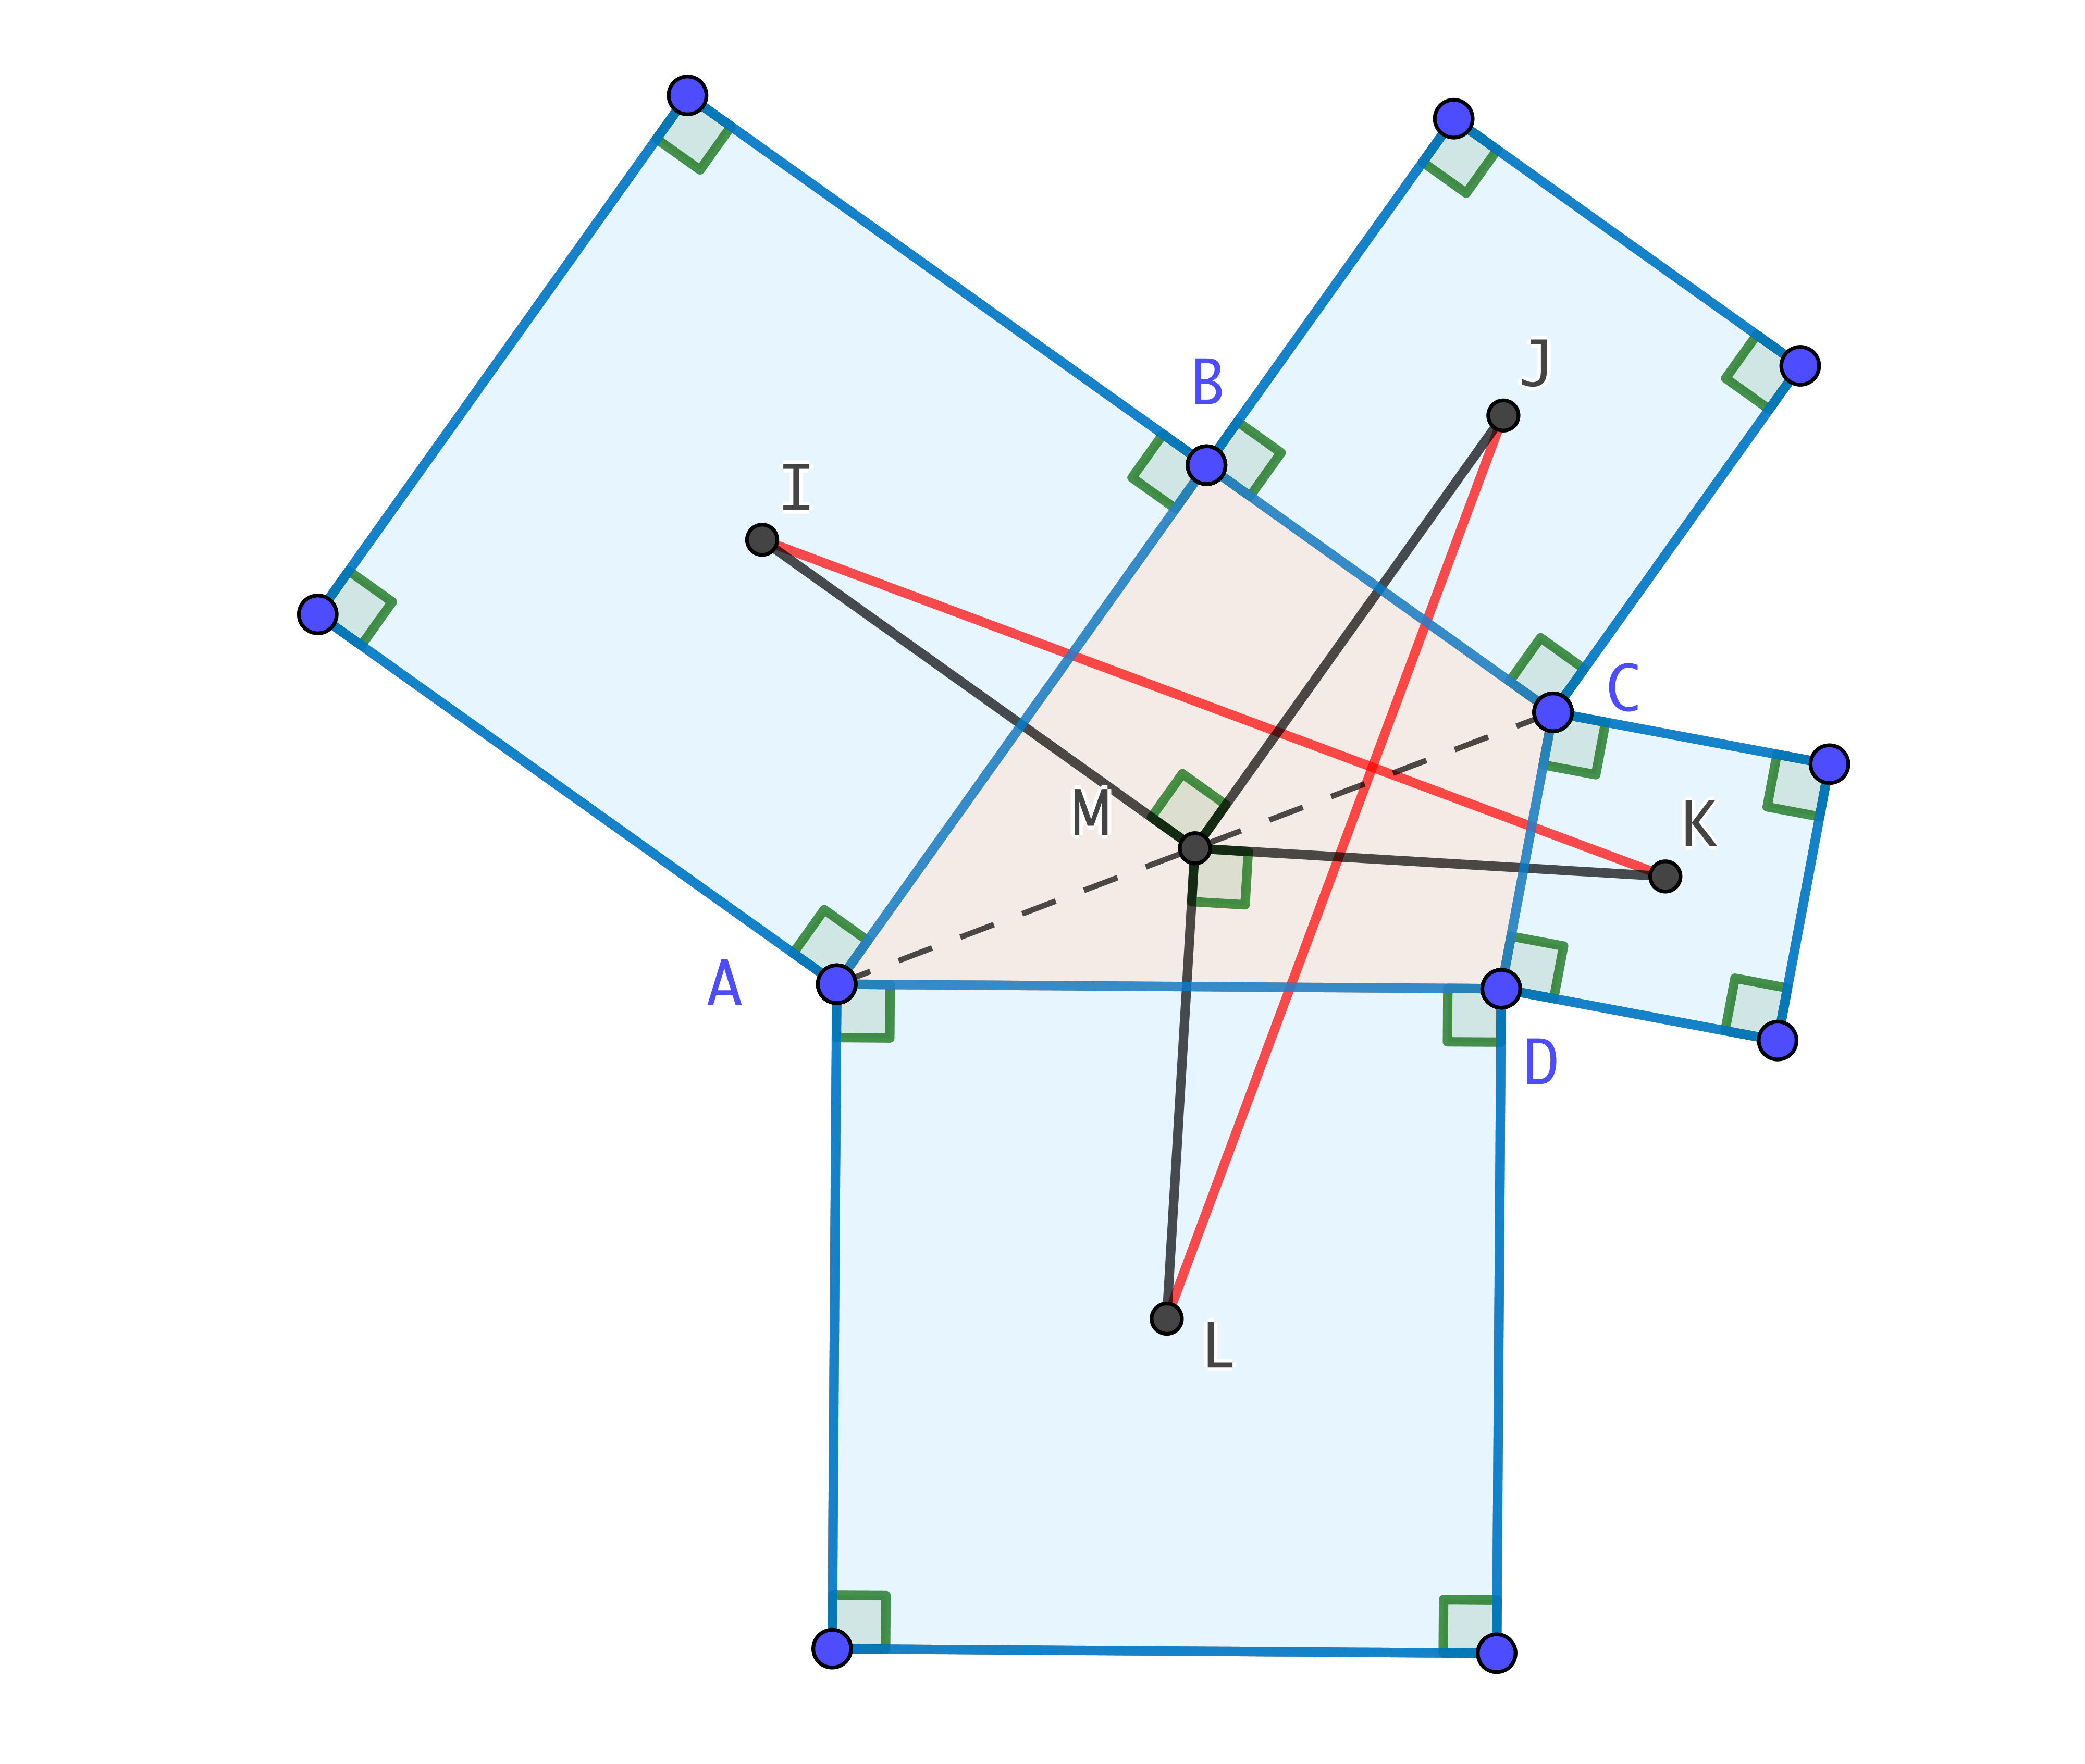
\includegraphics[scale=0.3]{todistus1}
\end{center}
Huomaamme, että kolmiot LMJ ja KMI ovat yhtenevät sillä molemmilla on kaksi samanpituista sivua IM, JM ja KM, LM, sekä niiden välillä suorakulma. Tästä seuraa, että sivut IK ja JL ovat myös yhtä pitkiä, näin ollaan todistettu osan lauseesta. Samaten siitä seuraa se että kulmat $\measuredangle$JLM ja $\measuredangle$IKM ovat yhtä suuret. Nimetään nämä kulmat $\alpha$ ja $\alpha'$.

Merkitään janojen JL ja KM leikkauspiste pisteellä N. Huomataan, että kulmat $\measuredangle$LNM ja $\measuredangle$JNK ovat ristikulmia eli yhtä suuret. Nimetään nämä kulmat $\beta$ ja $\beta'$.

\begin{center}
    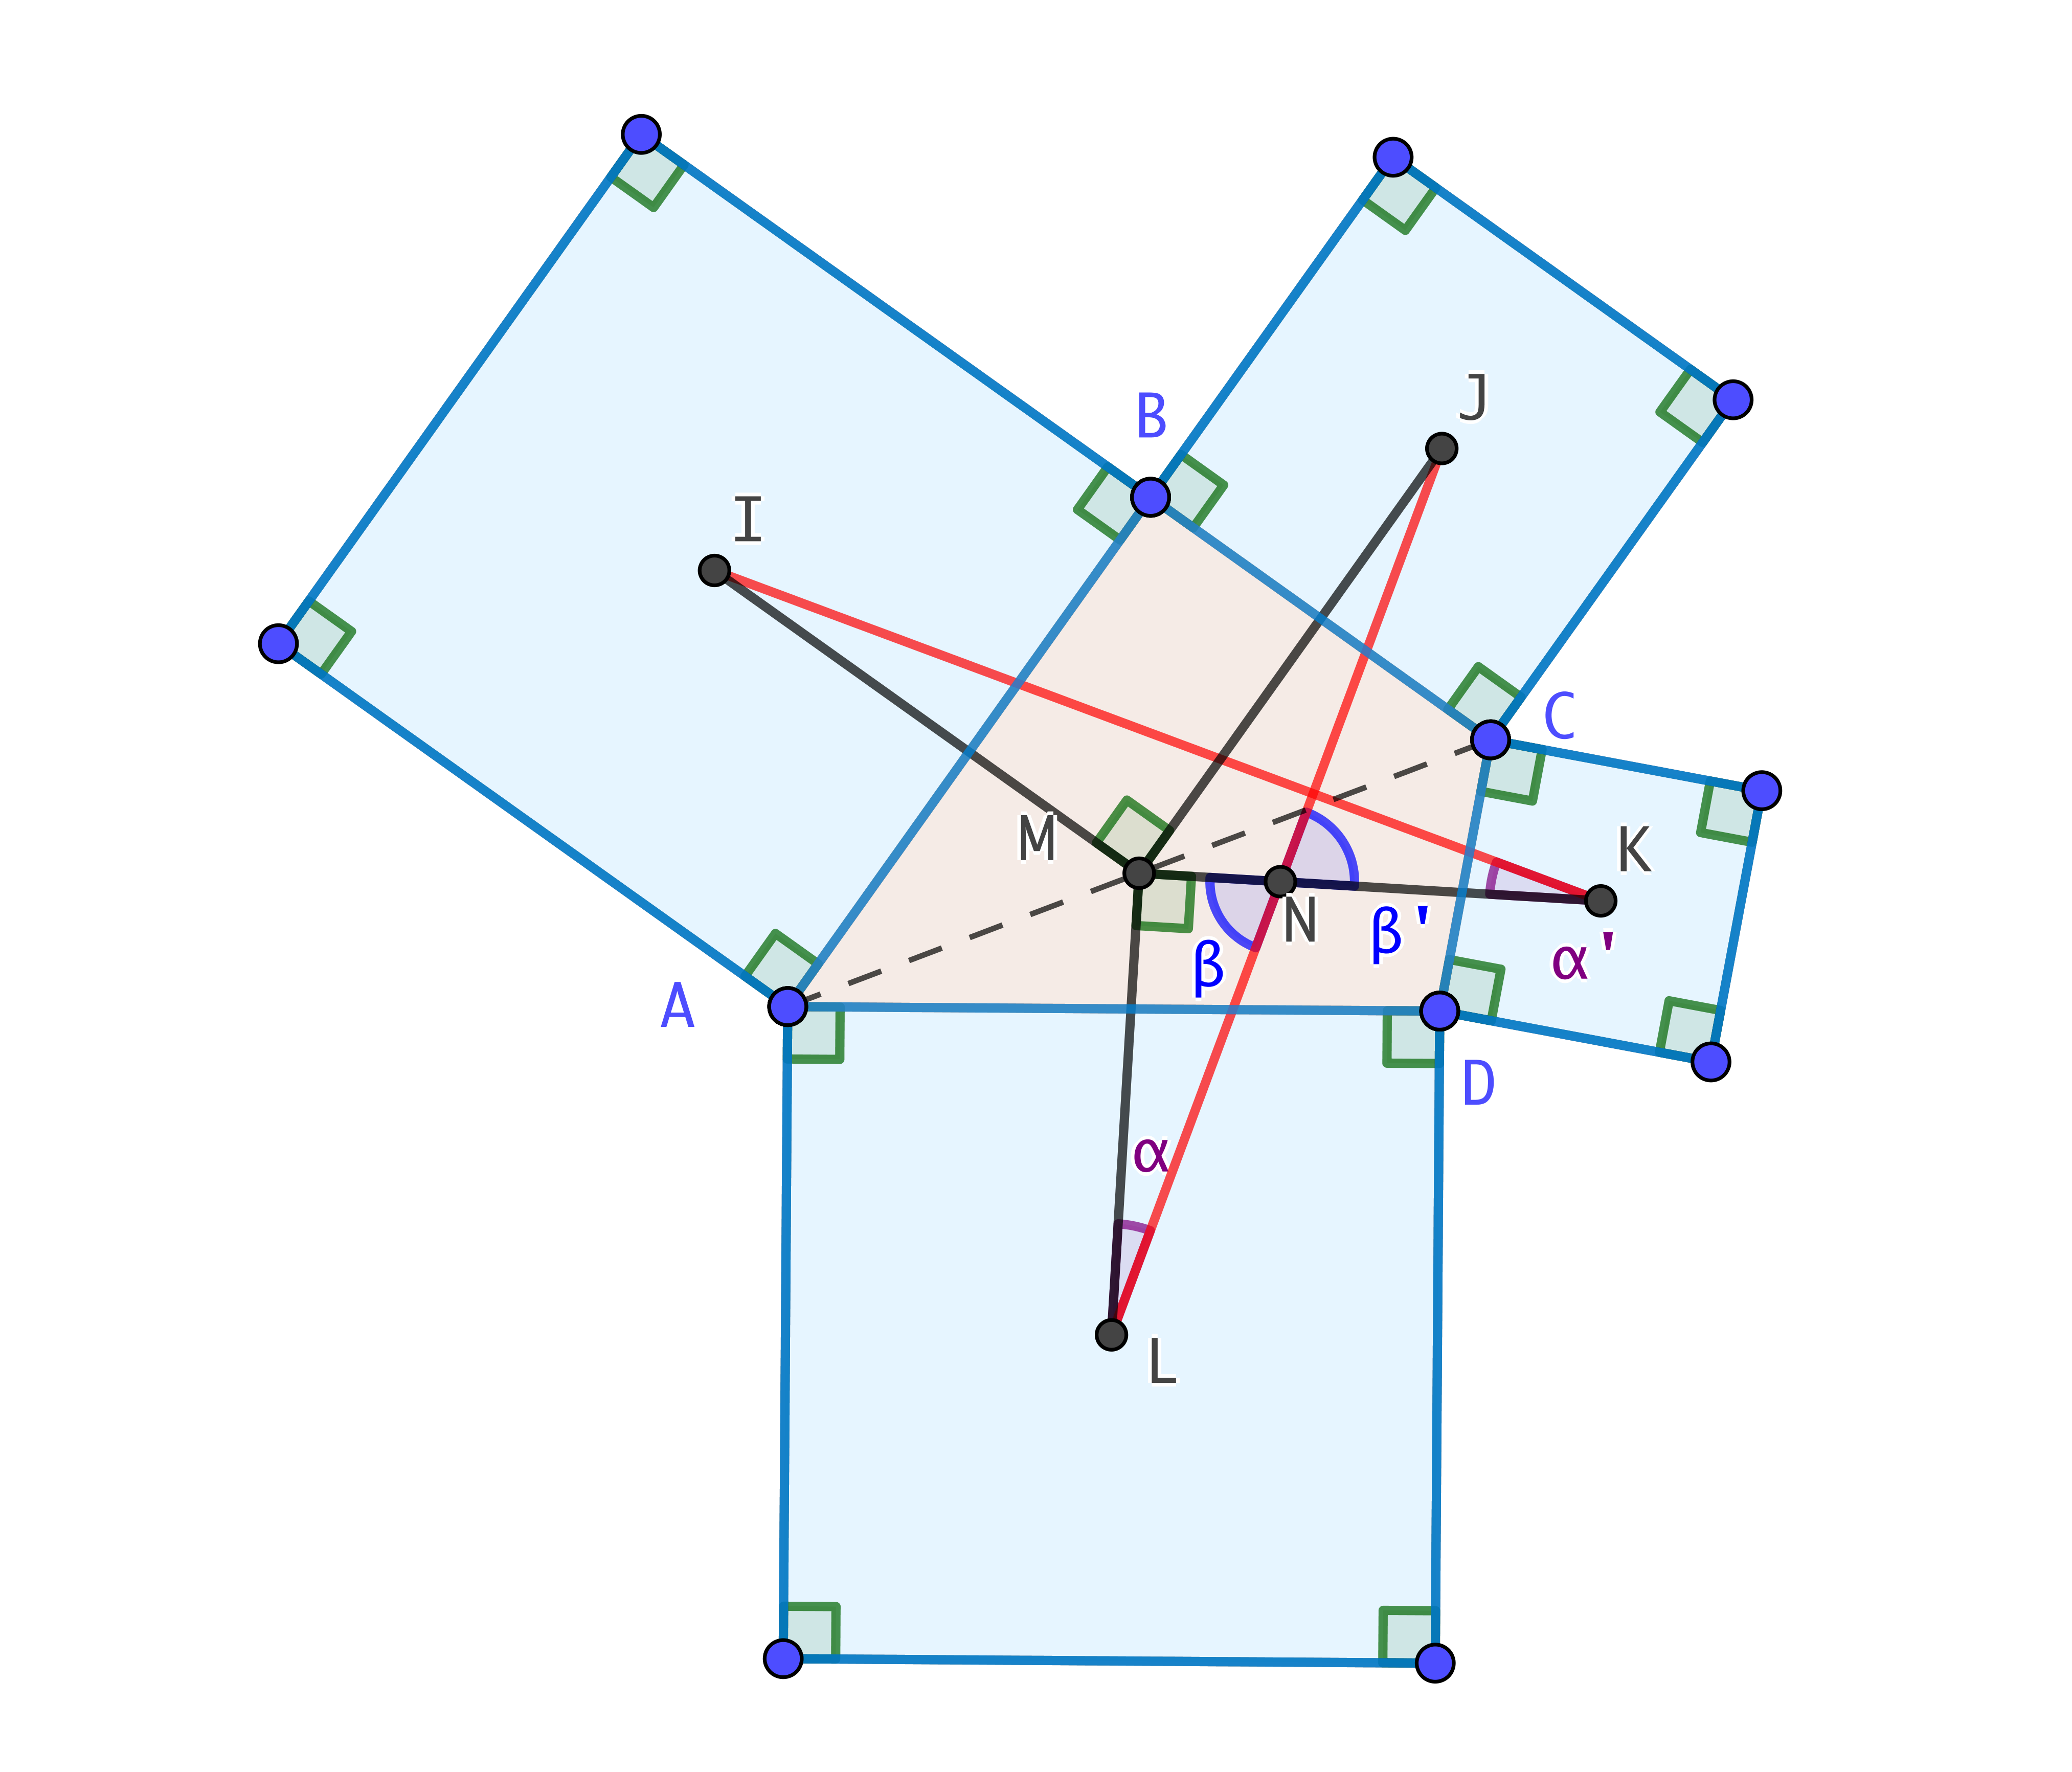
\includegraphics[scale=0.3]{todistuksenjatkoa.png}
\end{center}

Nyt nähdään, että $\alpha + \beta = 90^\circ$. Samaten myös $\alpha' + \beta' = 90^\circ$. Näin ollaan myös todistettu, että janat leikkaavat toisensa kohtisuorassa.

Tämä lause pätee, vaikka nelikulmio ei olisi konveksi, jos nelikulmion sivu kutistettaisiin pisteeksi sekä jos neliöt piirrettäisiin nelikulmion sisään.
%pitääkö tämäkin todistaa?

\pagebreak
\section{Sovellus}
%http://mathworld.wolfram.com/vanAubelsTheorem.html

Van Aubelin lauseen tapaisia lauseita ovat muun muassa Napoleonin lause sekä Petr–Douglas–Neumann teoreema.

Alkuperäisessä van Aubelin todistuksessa ei todistettu muuta kuin, että janat ovat yhtä pitkät ja kohtisuorassa toisiaan vastaan vaikka nelikulmio ei olisi konveksi eli nelikulmio voisi leikata itsensä. Lause pätee myös jos nelikulmion sivun kutistaisi pisteeksi tai jos nämä neliöt piirettäisiin nelikulmion sisään. 
%Kuvia tästä(????). 
Tämän lisäksi lauseella on muitakin ominaisuuksia, kuten se, jos neliöiden keskipisteet yhdistetään vierekkäisten neliöiden keskipisteiden kanssa, syntynyt nelikulmio on ortadiagonaalinen nelikulmio eli sen lävistäjät leikkaavat toisensa kohtisuorassa.

\pagebreak
\section{Lähteet}
van Aubel, H. H. (1878), "Note concernant les centres de carrés construits sur les côtés d'un polygon quelconque", Nouvelle Correspondance Mathématique (In French), 4: 40–44.

http://www.osaka-ue.ac.jp/zemi/nishiyama/math2010/aubel.pdf


\end{document}